\documentclass{beamer}
\input{../style/cours-style.sty}

% Title
\title[PYDATA]{Python - Data Scientist}
\author{Christophe Brun}
\institute{Digicomp}
\date{17 mai 2024}
\beamertemplatenavigationsymbolsempty

\titlegraphic{
    \bigbreak
    
\includegraphics[width=5cm]{image/digicomp-logo}
    \bigbreak
    Digital competence. Made of People.
    \bigbreak
}

\begin{document}

    \begin{frame}
        \titlepage
        \bigbreak
        \centering
        \url{https://github.com/DigicompClassesByPapIT/PYDATA}
    \end{frame}


    \section{Table des matières}\label{sec:toc}

    \begin{frame}{Table des matières}
        \begin{small}
            \begin{multicols}{2}
                \tableofcontents
            \end{multicols}
        \end{small}
    \end{frame}


    \section{Programme du module}\label{sec:programme-du-module}

    \begin{frame}{Python - Data Scientist}{Contenu des 2 jours}
        \begin{tiny}
            \begin{multicols}{3}
                \begin{itemize}
                {\tiny
                \item Programmation fonctionnelle
                    \begin{itemize}
                        \tiny
                        \item Expressions lambda
                        \item List comprehension
                    \end{itemize}

                    \item Jupyter Notebook
                    \begin{itemize}
                        \tiny
                        \item Fonctionnement local, serveur
                        \item Interface et commandes
                    \end{itemize}

                    \item NumPy
                    \begin{itemize}
                        \tiny
                        \item Création et manipulation de tableaux et matrices NumPy
                        \item Indexation et sélection
                        \item Manipulations arithmétiques, broadcasting
                        \item Fonctions statistiques
                    \end{itemize}

                    \item Pandas
                    \begin{itemize}
                        \tiny
                        \item Structures de données (Series, DataFrame, Panel)
                        \item Indexation et sélection
                        \item Fonctions statistiques
                        \item Combinaison des données (concat, append, merge, join)
                        \item Fenêtrage
                        \item Groupement et agrégation
                        \item Données temporelles
                    \end{itemize}

                    \item Chargement et sauvegarde des données
                    \begin{itemize}
                        \tiny
                        \item Traitement des principaux formats de fichiers
                        \begin{itemize}
                            \tiny
                            \item Excel, CSV, XML, JSON
                        \end{itemize}
                        \item Requêtes SQL avec Pandas
                    \end{itemize}

                    \item Préparation et nettoyage des données
                    \begin{itemize}
                        \tiny
                        \item Traitement des données manquantes
                        \item Combinaison et transformation de données
                        \item Agrégation et regroupement de données
                        \item Traitement des données temporelles
                    \end{itemize}

                    \item Visualisation avec Matplotlib, Seaborn et Plotly
                    \begin{itemize}
                        \tiny
                        \item Types de graphiques
                        \begin{itemize}
                            \tiny
                            \item Ligne, point, histogramme, bar, pie, \ldots{}
                        \end{itemize}
                        \item Label, légende, grille, axes, titre
                        \item Sauvegarde des graphiques
                        \item Visualisation avec Seaborn
                        \item Visualisation web interactive avec Plotly
                    \end{itemize}

                    \item Exemple d'analyse de données financières

                    \item Introduction au Machine Learning
                }
                \end{itemize}
            \end{multicols}
        \end{tiny}

    \end{frame}


    \section{Introduction}\label{sec:introduction}

    \begin{frame}{Formateur sur Linux}{Christophe Brun, conseil en développement informatique}

        \begin{columns}
            \column{0.7\textwidth}
            \begin{itemize}
                \item Développeur freelance (Python, Java, CoBOL) et data at scale.

                \item 7 ans de conseil en développement au sein d'SSII~.

                \item 8 ans de conseil en développement en indépendant, \href{https://papit.fr}{PapIT}.

                \item Passionné~!
                \bigbreak
                \begin{columns}
                    \column{0.5\textwidth}
                    \centering
                    
\includegraphics[width=3cm]{image/logo-uppa}
                    \column{0.5\textwidth}
                    \centering
                    
\includegraphics[width=3cm]{image/logo-universite-bordeaux}
                \end{columns}
            \end{itemize}
            \column{0.3\textwidth}
            \centering
            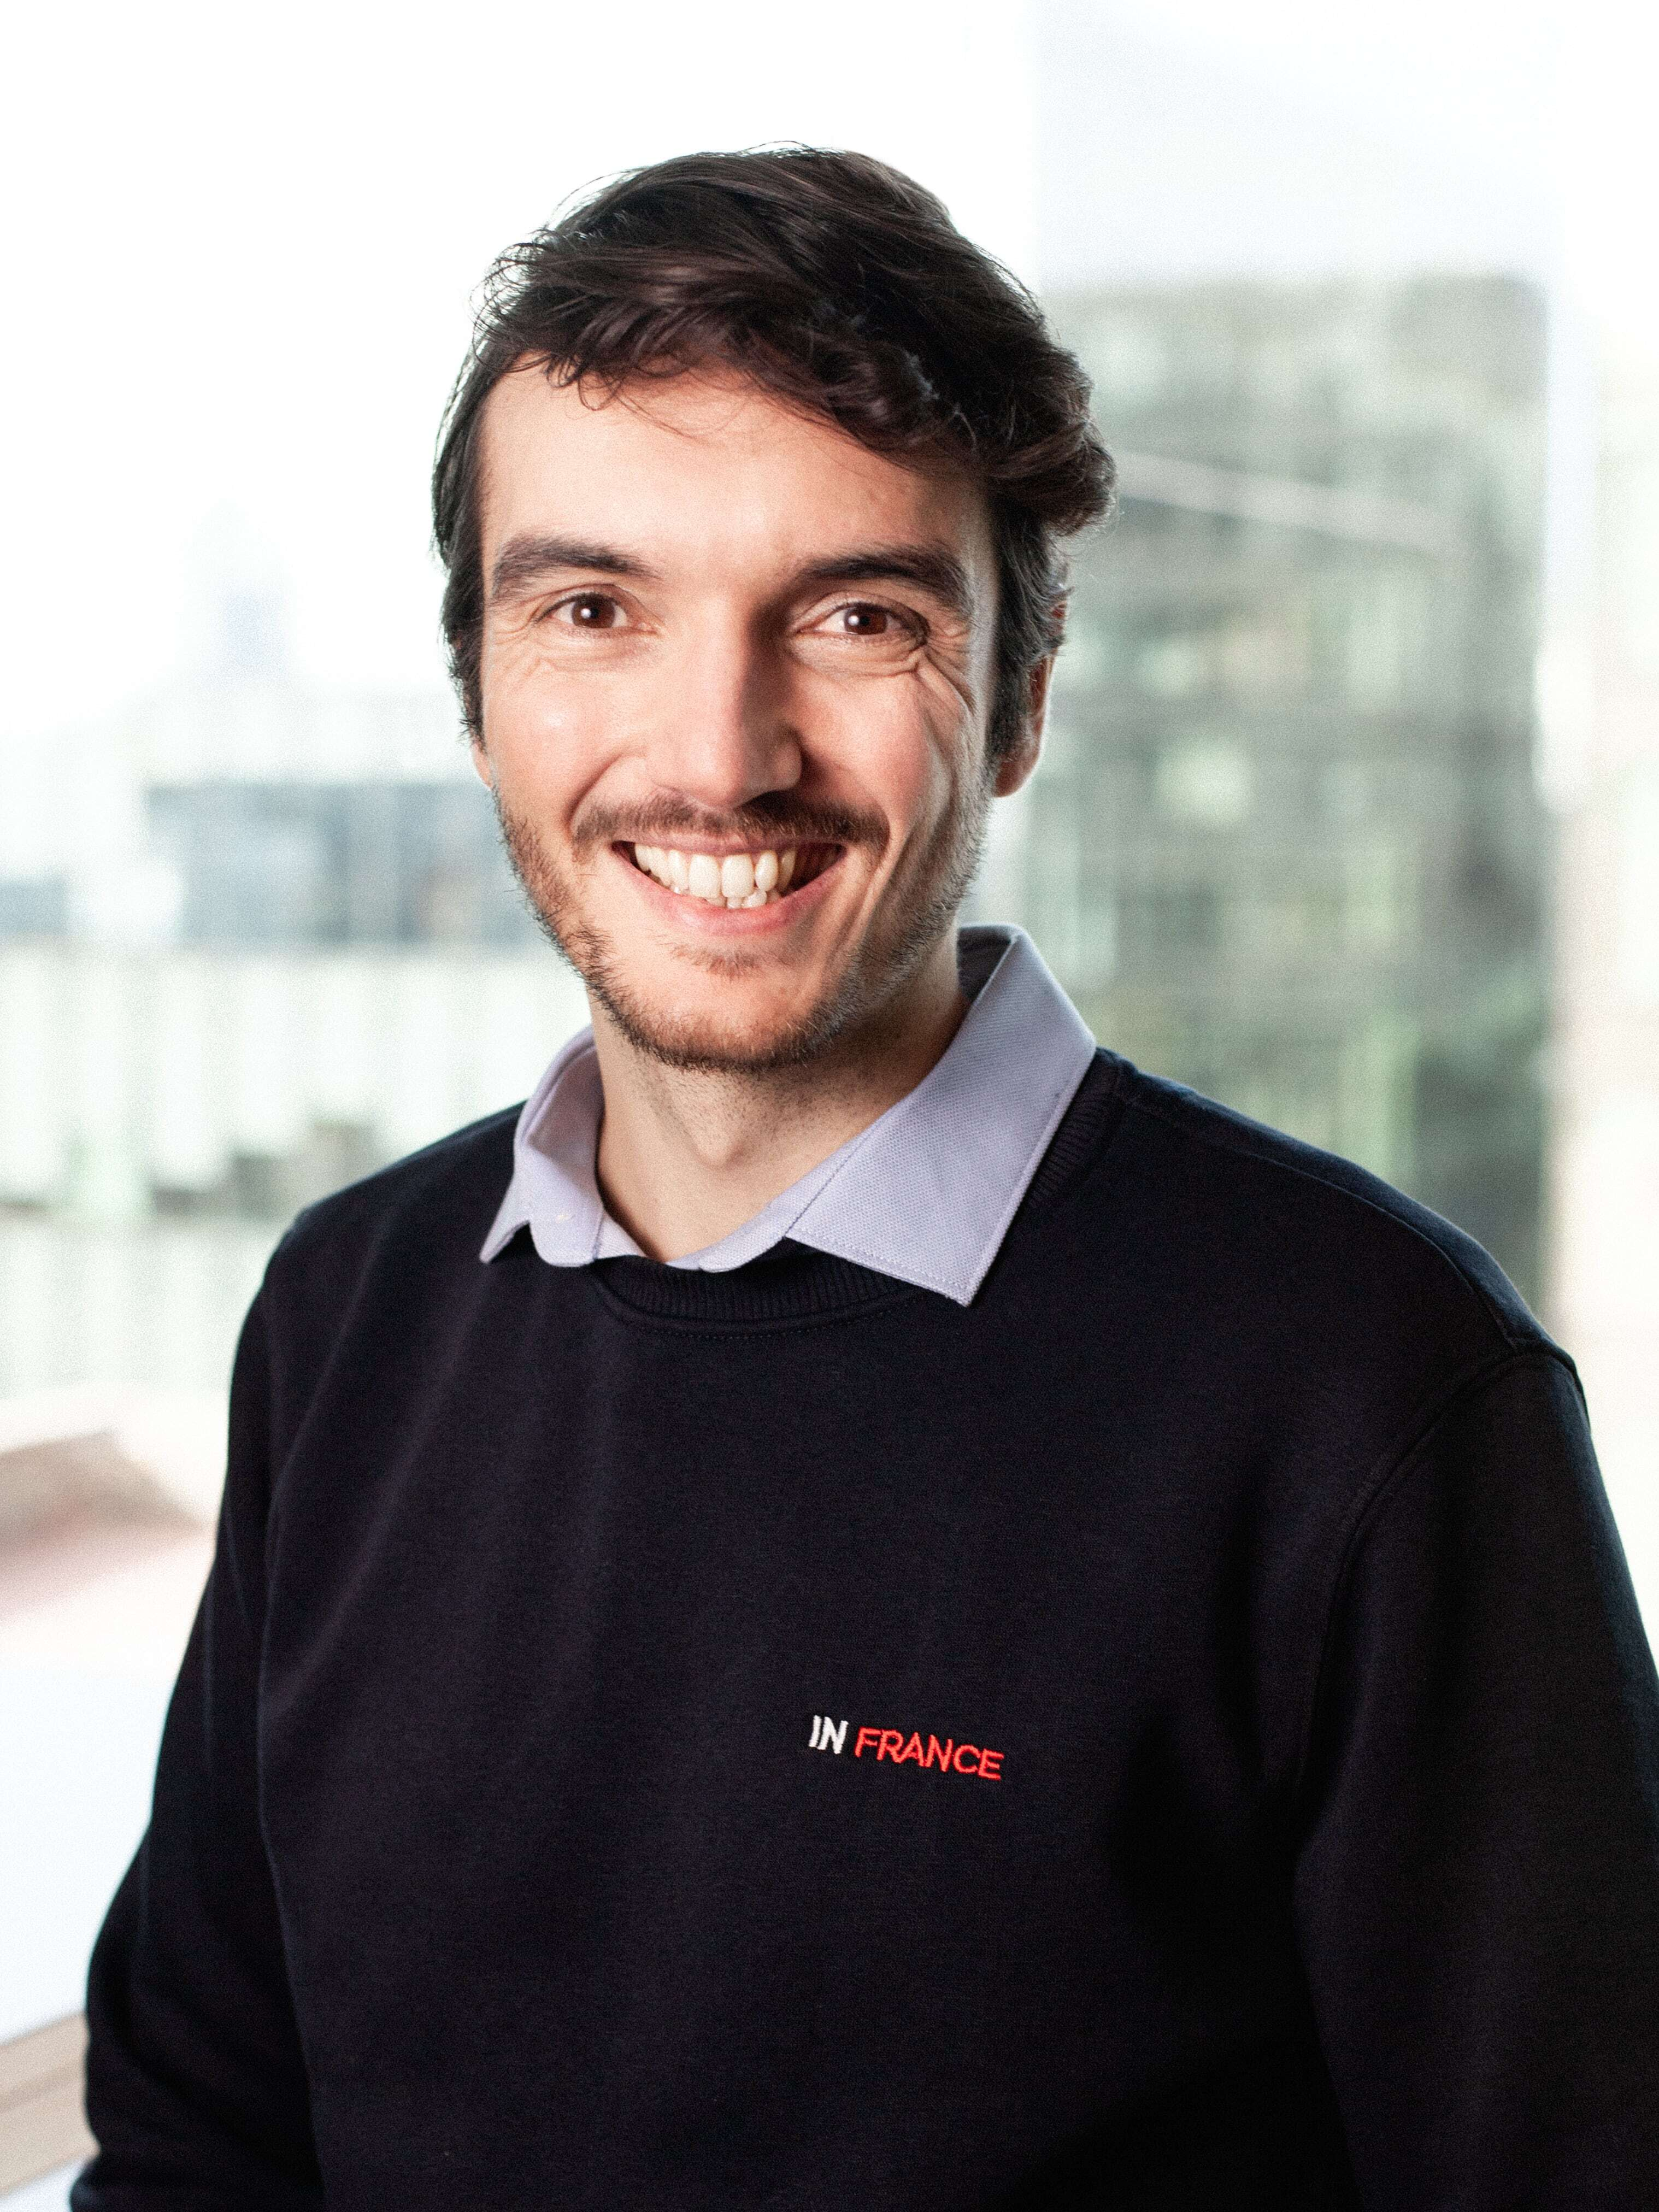
\includegraphics[width=5cm]{image/trombine-christophe}
        \end{columns}
    \end{frame}


    \section{Machine Learning}\label{sec:ml}

    \begin{frame}{Machine Learning}{Les librairies}
        Python est le langage de la Data Science et du Machine Learning.
        Il surpasse depuis des années l'écosystème \href{https://posit.co/download/rstudio-desktop/}{R}.
        \bigbreak
        Mais la Data Science nécessite de nombreuses librairies, les plus connues sont~:
        \begin{itemize}
            \item \href{https://numpy.org/}{NumPy} pour les calculs scientifiques
            \item \href{https://pandas.pydata.org/}{Pandas} pour la manipulation de données
            \item \href{https://matplotlib.org/}{Matplotlib} pour la visualisation de données
            \item \href{https://plotly.com/}{Plotly} pour la visualisation de données
            \item \href{https://scikit-learn.org/stable/}{Scikit-learn} pour le Machine Learning
            \item \href{https://www.tensorflow.org/}{TensorFlow} pour le Deep Learning
            \item \href{https://pytorch.org/}{PyTorch} pour le Deep Learning
        \end{itemize}
    \end{frame}

    \begin{frame}{Machine Learning}{Régression linéaire avec Scikit-learn}
        Télécharger et ouvrir le notebook \url{https://github.com/DigicompClassesByPapIT/Python/blob/main/15_simple_linear_regression}.
        Ce dernier illustre un exemple de régression linéaire simple avec Scikit-learn.
        \bigbreak
        \begin{columns}
            \column{0.5\textwidth}
            La regression linéaire est un des plus simples algorithmes de Machine Learning.
            Il permet de prédire une variable continue à partir d'une autre variable continue en trouvant la meilleure droite qui les relie.
            Celle qui a le R carré le plus élevé, le plus proche de 1.
            \column{0.5\textwidth}
            \centering
            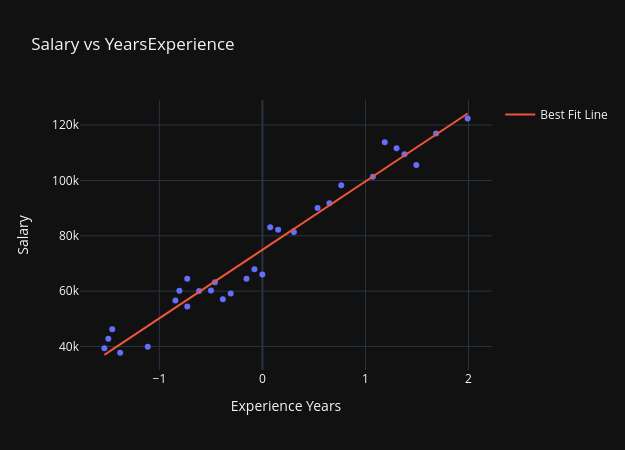
\includegraphics[width=6cm]{image/linear-regression}
        \end{columns}
        \bigbreak
        Le salaire est la variable \textit{target} qui pourra être prédite à partir de l'expérience la variable année d'expérience, la \textit{feature}.
    \end{frame}

    \begin{frame}{Machine Learning}{Régression linéaire avec Scikit-learn}
        Avec la méthode \lstinline{train_test_split} de Scikit-learn on peut diviser les données en deux jeux~:
        \begin{itemize}
            \item Un jeu d'entraînement pour entraîner le modèle et trouver la meilleure regression linéaire
            \item Un jeu de test pour tester le modèle et calculer le R carré et d'autres métriques, sur un jeu de données inconnues.
        \end{itemize}
        \begin{dangercolorbox}
            Le Machine Learning n'est qu'un domaine de la Data Science.
            Il a besoin des mêmes outils pour le pré-traitement des données (A.K.A \textit{data wrangling}), la visualisation, la manipulation, \textit{etc}.
            Pour ce faire il faut maîtriser les librairies \lstinline{pandas}, \lstinline{plotly}.
            \lstinline{pandas} est une librairie très puissante pour la manipulation de données, elle est très utilisée en Data Science.
            Elle n'est pas compliquée mais mériterait une journée de formation à elle seule.
            Regardez les notebook \url{https://github.com/jupyter-naas/awesome-notebooks/tree/master/Pandas} pour vous autoformer.
        \end{dangercolorbox}
    \end{frame}

    \begin{frame}{Machine Learning}{Régression linéaire avec Scikit-learn}
        Exercice \execcounterdispinc{}, créer un notebook et étudier le dataset \url{https://github.com/DigicompClassesByPapIT/Python/blob/main/advertising.csv}.
        Il contient les données de ventes en fonction de la publicité TV, radio et journaux.
        \bigbreak
        La variable \textit{target} est les ventes, les \textit{features} sont les budgets publicitaires.
        Trouver quelle est la meilleure \textit{feature} de prédiction des ventes, celle qui a le R carré le plus élevé.
    \end{frame}


    \section{Licence CC}\label{sec:licence}

    \begin{frame}{Licence}{Licence Creative Commons}
        Support de cours sous licence Creative Commons BY-NC-ND~.
        \bigbreak
        Vous pouvez donc, partager, copier, distribuer le document.
        \bigbreak
        Attribution requise à PapIT SASU - Pas d’utilisation commerciale - Pas de modification
        \bigbreak
        \centering
        
\includegraphics[width=5cm]{image/by-nc-nd-logo}
    \end{frame}


\end{document}
